\documentclass[12pt]{kiarticle} % You can learn about my document class "kiarticle" and install it to your device by following the link: https://github.com/Kiarendil/toolkitex
\graphicspath{{pictures/}}
\DeclareGraphicsExtensions{.pdf,.png,.jpg,.eps}
%%%
\pagestyle{fancy}
\fancyhf{}
%\renewcommand{\headrulewidth}{ 0.1mm }
\renewcommand{\footrulewidth}{ .0em }
\fancyfoot[C]{\texttt{\textemdash~\thepage~\textemdash}}
\fancyhead[L]{Лабораторная работа № 3.4.5 \hfil}
\fancyhead[R]{\hfil Иванов Кирилл, 625 группа }
\usepackage{multirow} % Слияние строк в таблице
\newcommand
{\un}[1]
{\ensuremath{\text{#1}}}
\newcommand{\eds}{\ensuremath{ \mathscr{E}}}
\usepackage{tikz}

\begin{document}
		
		\begin{titlepage}
			\begin{center}
				\large 	Московский физико-технический институт \\
				Факультет общей и прикладной физики \\
				\vspace{0.2cm}
				
				\vspace{4.5cm}
				Лабораторная работа № 3.4.5 \\ \vspace{0.2cm}
				\large (Общая физика: электричество и магнетизм) \\ \vspace{0.2cm}
				\LARGE \textbf{Петля гистерезиса (динамический метод)}
			\end{center}
			\vspace{2.3cm} \large
			
			\begin{center}
				Работу выполнил: \\
				Иванов Кирилл,
				625 группа
				\vspace{10mm}		
				
			\end{center}
			
			\begin{center} \vspace{60mm}
				г. Долгопрудный \\
				2017 год
			\end{center}
		\end{titlepage}

	
	\paragraph*{Цель работы:} изучение петель гистерезиса ферромагнитных материалов с помощью осциллографа.
	
	\paragraph*{Оборудование:} автотрансформатор, понижающий трансформатор, амперметр и вольтметр (мультиметры), резистор, делитель напряжения, интегрирующая
	цепочка, электронный осциллогра, тороидальные образцы с двумя обмотками..
	
	\section{Теоретическое введение}
	
	\begin{wrapfigure}{l}{0.6\textwidth}
		\vspace{-20pt}
		\begin{center}
			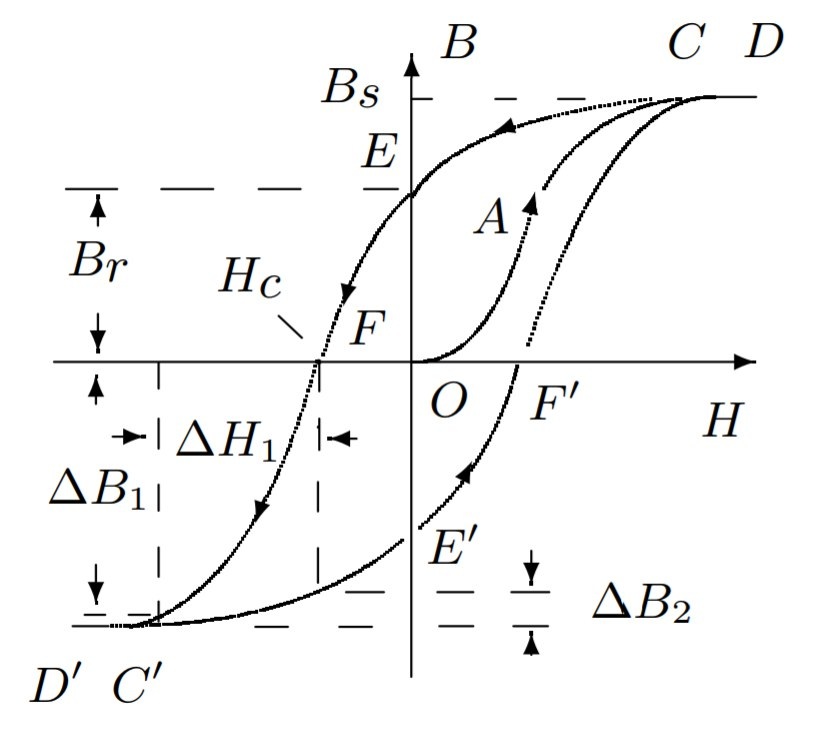
\includegraphics[width=0.7\linewidth]{gist3.jpg}
			\label{fig:sdfsafd}
		\end{center}
		\vspace{-10pt}
		\caption{Петля гистерезиса ферромагнетика}
	\end{wrapfigure}

	Магнитная индукция $\vec{B}$ и напряженность магнитного поля
	$\vec{H}$ в ферромагнитном материале неоднозначно связаны
	между собой: индукция зависит не только от напряженности, но
	и от предыстории образца. Связь между индукцией
	и напряженностью поля типичного ферромагнетика иллюстрирует рис. 1. Если
	к размагниченному образцу начинают прикладывать магнитное поле, то его намагничивание следует кривой $ OACD $, выходящей
	из начала
	координат. Эту кривую называют \textit{основной кривой намагничивания}.
	
	
	Индукция $\vec{B}$ в образце состоит из индукции, связанной с намагничивающим полем
	$\vec{B}$, и индукции, создаваемой самим намагниченным
	образцом.
	В системе СИ эта связь имеет вид
	
	$$\vec{B} = \mu_{0}(\vec{H}+\vec{M}),$$
	
	где $\vec{M}$- \textit{намагниченность} - магнитный момент единичного объема образца, а $\mu_{0}$ - магнитная постоянная.
	
	Намагнитим образец до насыщения - до точки D. Соответствующее
	значение индукции $B_{s}$ называют индукцией насыщения. При уменьшении поля $H$ до нуля зависимость $B(H)$ имеет вид кривой $DCE$, и при нулевом поле индукция имеет конечное ненулевое значение. Это остаточная индукция $B_{r}$ . Чтобы размагнитить образец, то есть перевести его в состояние
	$F$, необходимо приложить "обратное" магнитное
	поле $H_{c}$, которое называют коэрцитивной силой.
	
	Замкнутая кривая $DEFD'E'F'D$, возникающая при циклическом
	перемагничивании образца, намагниченного до насыщения, называется \textit{предельной петлей гистерезиса.}
	
	
	\subsection{Измерение магнитной индукции в образцах.}
	Магнитную индукцию удобно определять с помощью ЭДС, возникающей при изменении магнитного потока Ф в катушке, намотанной на образец:
	
	$$\mathscr{E} = -\dfrac{dФ}{dt}.$$
	
	Тогда отсюда и из формулы $Ф=BSN_{и}$ получаем:
		$$|B|=\dfrac{1}{SN_{и}}\int \mathscr{E}dt.$$
	Для интегрирования сигнала применяют интегрирующие схемы (рис. 2).
	
		\begin{wrapfigure}{l}{0.6\textwidth}
		\vspace{-20pt}
		\begin{center}
			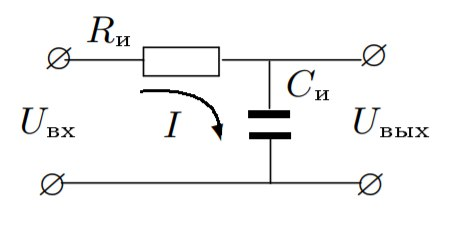
\includegraphics[width=0.7\linewidth]{gist2.jpg}
			\label{fig:sdfsafd}
		\end{center}
		\vspace{-10pt}
		\caption{Интегрирующая RC-цепь}
	\end{wrapfigure}
	
	Если выходной сигнал намного меньше входного ($U_{вых}\ll U_{вх},$) ток в цепи пропорционален входному напряжению: $I\simeq\dfrac{U_{вх}}{R}$, а напряжение на емкости С
	
	$$U_{вых}\simeq\dfrac{1}{RС}\int U_{вх}dt.$$
	
	Этот вывод тем ближе к истине, чем больше постоянная $\tau=RC$ превосходит характерное время процесса (например, его период). Для синусоидальных напряжений
	
	$$U_{вых}=\dfrac{U_{вх}}{RC\Omega},$$
	
	где $\Omega$ - частота сигнала.
	
	В итоге, обозначив параметры интегрирующей цепи через $R_{и}$ и $C_{и}$, получаем
	
	$$ |B|=\dfrac{1}{SN_{и}}\int U_{вх}dt=\dfrac{R_{и}С_{и}}{SN_{и}}U_{вых}.$$
	
	\section{Экспериментальная установка.}
	Схема экспериментальной установки показана на рис. 3.
	
	Действующее значение переменного тока в обмотке N0 измеряется амперметром А (мультиметром GDM). Последовательно с амперметром включено сопротивление $R_{0}$, напряжение с которого подается на вход X электронного осциллографа (ЭО). Это напряжение пропорционально току в обмотке $N_{0}$, а следовательно и напряженности H магнитного поля в образце.
	
	Для измерения магнитной индукции B с измерительной обмотки $N_{И}$ на вход интегрирующей RC -цепочки подается напряжение $U_{И}$ (UВХ), пропорциональное производной $\dot{B}$, а с выхода снимается напряжение $U_{C}$($U_{ВЫХ}$), пропорциональное
	величине B , и подается на вход Y осциллограа.
	Замкнутая кривая, возникающая на экране, воспроизводит в некотором масштабе (различном для осей X и Y ) петлю гистерезиса. Чтобы придать этой кривой количественный смысл, необходимо установить масштабы изображения, т.е. провести калибровку каналов X и Y ЭО. Для этого, во-первых, надо узнать, каким напряжениям (или токам) соответствуют амплитуды сигналов, видимых на экране, и во-вторых,  каким значениям B и H соответствуют эти напряжения
	(или токи).
	
	\begin{figure}[h!]
		\centering
		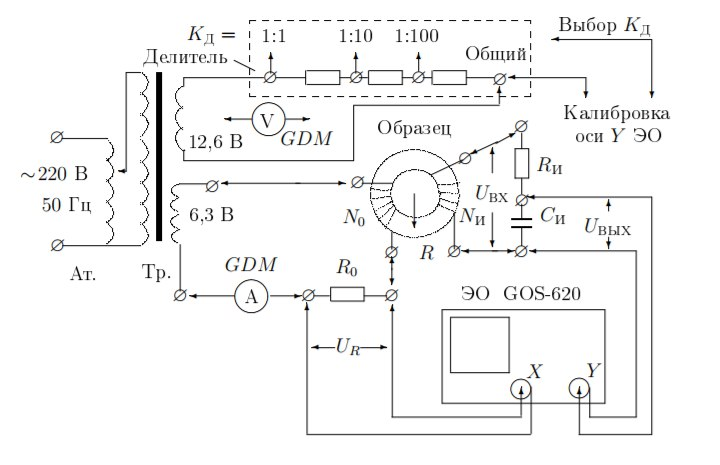
\includegraphics[width=\linewidth]{gist.jpg}
		\caption{Схема установки для исследования намагничивания образцов}
		\label{fig:Holl2}
	\end{figure}
  
  	
  	\section{Ход работы}
  	
  	\begin{enumerate}
  	\item Запишем данные установки:
  	
  	$R_{0}=0,2 Ом \ \ R_{и}=20 кОм \ \ С_{и}=20 мкФ $
  	
  	Параметры тороидальных образцов:
  	
  \begin{itemize}
  	\item 	\textbf{Кремниевое железо $ Fe-Si $}: 
  	$N_{0}=20$ витков;
  	$N_{и}=200$ витков;
  	$S=2 см^{2}$;
  	$2\pi R = 11 см $. 
  	
  \item	\textbf{Пермаллой $ Fe-Ni $  НП50}: $N_{0}=15$ витков;
  	$N_{и}=300$ витков;
  	$S=0,66 см^{2}$;
  	$2\pi R = 14,1 см $.  
  	
  \item	\textbf{Феррит 1000нн}: $N_{0}=45$ витков;
  			$N_{и}=400$ витков;
  			$S=3,0 см^{2}$;
  			$2\pi R = 25 см $.  
  \end{itemize}
  
  	 
  	\item Соберем схему (рис. 3) и настроим оборудование. 	
 
 	\item Для каждого образца сфотографируем предельную петлю. Запишем значения коэффициентов усиления $K_{x}$ и $K_{y}$, ток $I_{эф}$. Измерим двойные амплитуды для коэрцитивной силы $2x(c)$ и индукции насыщения $2y(s)$. Результаты таковы:
 	
 	 \begin{itemize}
 	 	\item 	\textbf{Кремниевое железо}:
 	
 	$K_{x}=100 \dfrac{мВ}{дел},$
 	$K_{y}=20 \dfrac{мВ}{дел},$
 	$I_{эф}=1,03 А. $
 	При этом $ 2x = 6,2 дел, \; 2y = 6,8 дел$.
 	
 \item 	\textbf{Пермаллой}:
 	
 	$K_{x}=20 \dfrac{мВ}{дел},$
 	$K_{y}=50 \dfrac{мВ}{дел},$
 	$I_{эф}=218 мА. $
 	При этом $ 2x = 7 дел, \; 2y = 3,5 дел$.
 	
 \item 	 \textbf{Феррит}:
 	 
 $K_{x}=10 \dfrac{мВ}{дел},$
 $K_{y}=50 \dfrac{мВ}{дел},$
 $I_{эф}=92,6 мА. $
 При этом $ 2x = 7,1 дел, \; 2y = 8 дел$.
  	
  
  	
 	 \end{itemize}

  	
  	
  	\item Снимем для каждого образца начальную кривую намагничивания (табл. 1-3), плавно уменьшая ток до нуля и отмечая вершины частных петель. По этим данным построим эти кривые (рис. 4-6).
  	
  		\begin{table}[h!]
  		\caption{Начальная кривая намагничивания для кремнистого железа}
  		\begin{center}
  			\begin{tabular}{|c|c|c|c|c|c|c|c|c|c|c|c|c|c|} 
  				\hline 
  				№ &  1 &  2 & 3 & 4 & 5 &  6 &  7 & 8 & 9 & 10  &  11 &  12 & 13  \\ 	\hline
  				
  			 $ x $, дел & 2.0 & 1.8 & 1.6 & 1.5 & 1.4 & 1.2 & 1.0 & 0.8 & 0.6 & 0.5 & 0.4 & 0.2 & 0.0 \\
  				 $ y $, дел & 3,0 & 2.8 & 2.7 & 2.5 & 2.3 & 2.1 & 2 & 1.6 & 1.2 & 0.7 & 0.4 & 0.1 & 0.0 \\
  				\hline
  				
  			\end{tabular}
  		\end{center}
  	\end{table}
  	
  	\begin{figure}[h!]
  		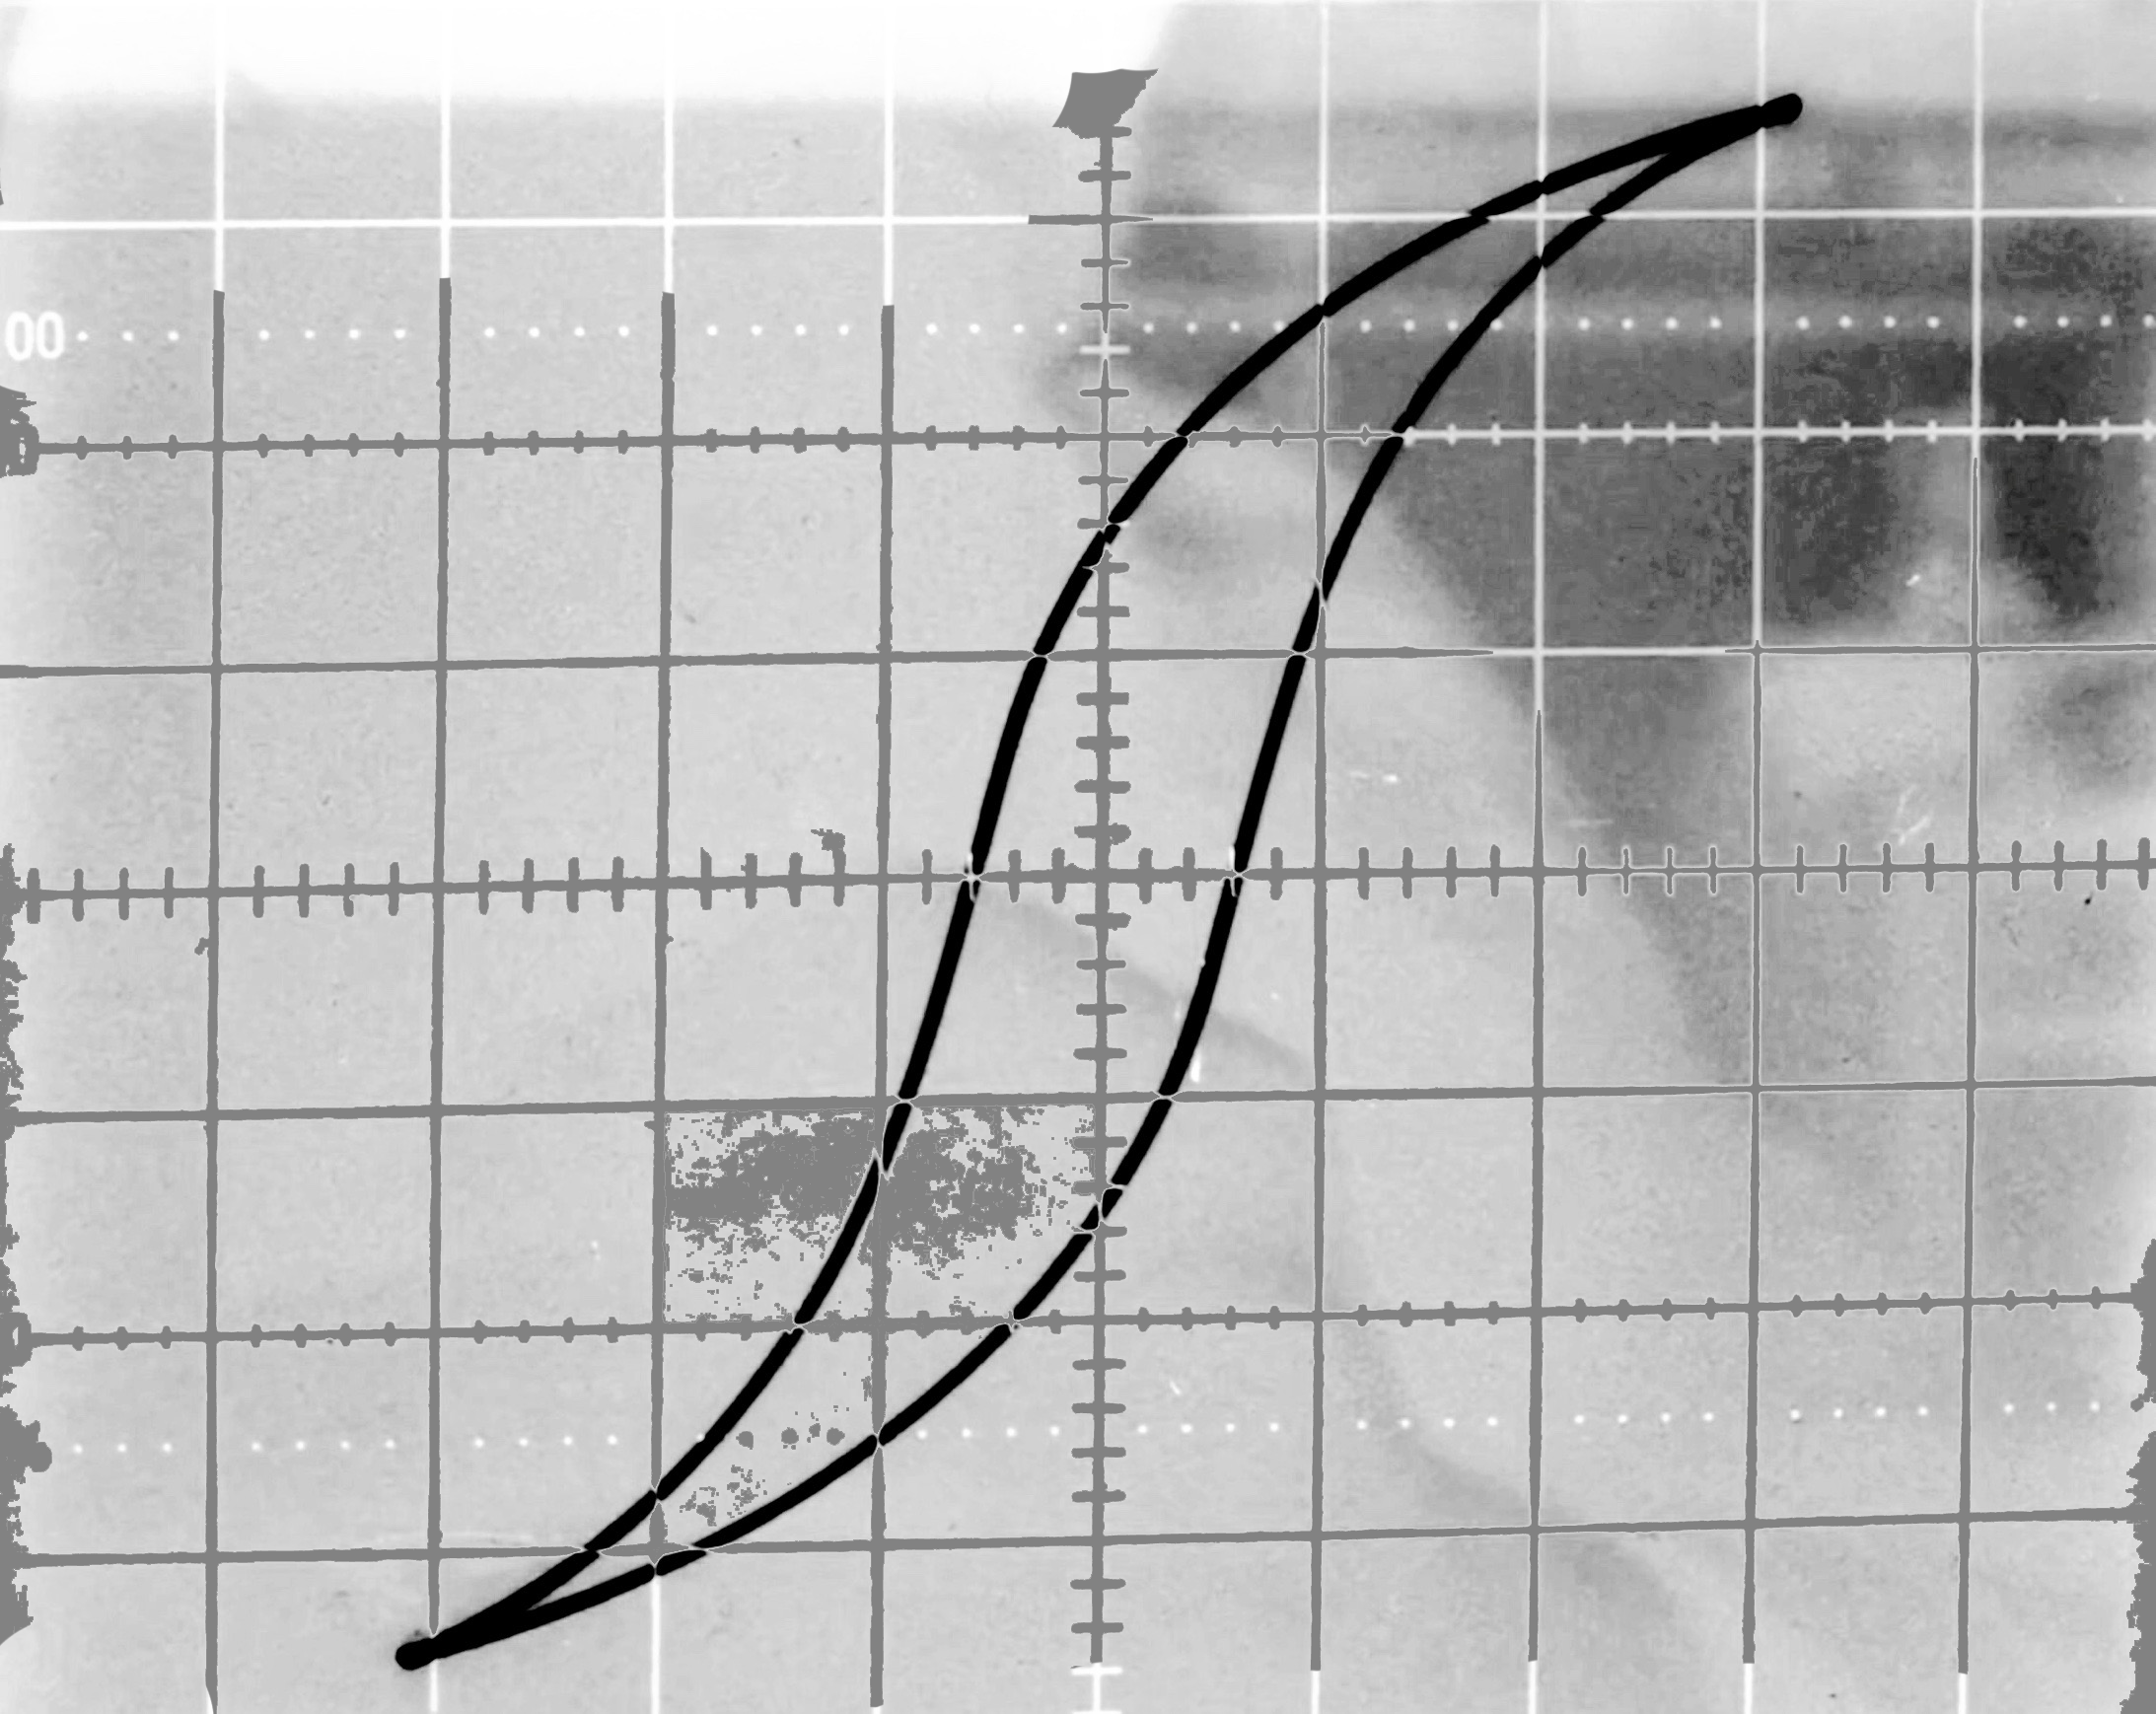
\includegraphics[scale=0.22]{1.png}
  		\caption{Петля гистерезиса для кремнистого железа}
  	\end{figure}
  


		\begin{table}[h!]
		\caption{Начальная кривая намагничивания для пермаллоя}
		\begin{center}
			\begin{tabular}{|c|c|c|c|c|c|c|c|c|c|c|c|c|c|} 
				\hline 
				№ &  1 &  2 & 3 & 4 & 5 &  6 &  7 & 8 & 9 & 10  &  11 &  12 &13   \\ 	\hline
				
			$ x $, дел & 3.0 & 2.8 & 2.6 & 2.4 & 2.2 & 2.0 & 1.8 & 1.5 & 1.2 & 0.8 & 0.5 & 0.2 & 0.0 \\
			 $ y $, дел & 1.8 & 1.7 & 1.5 & 1.4 & 1.1 & 1 & 0.9 & 0.7 & 0.5 & 0.4 & 0.2 & 0.1 & 0.0 \\
				\hline
				
			\end{tabular}
		\end{center}
	\end{table}


	\begin{figure}[h!]
	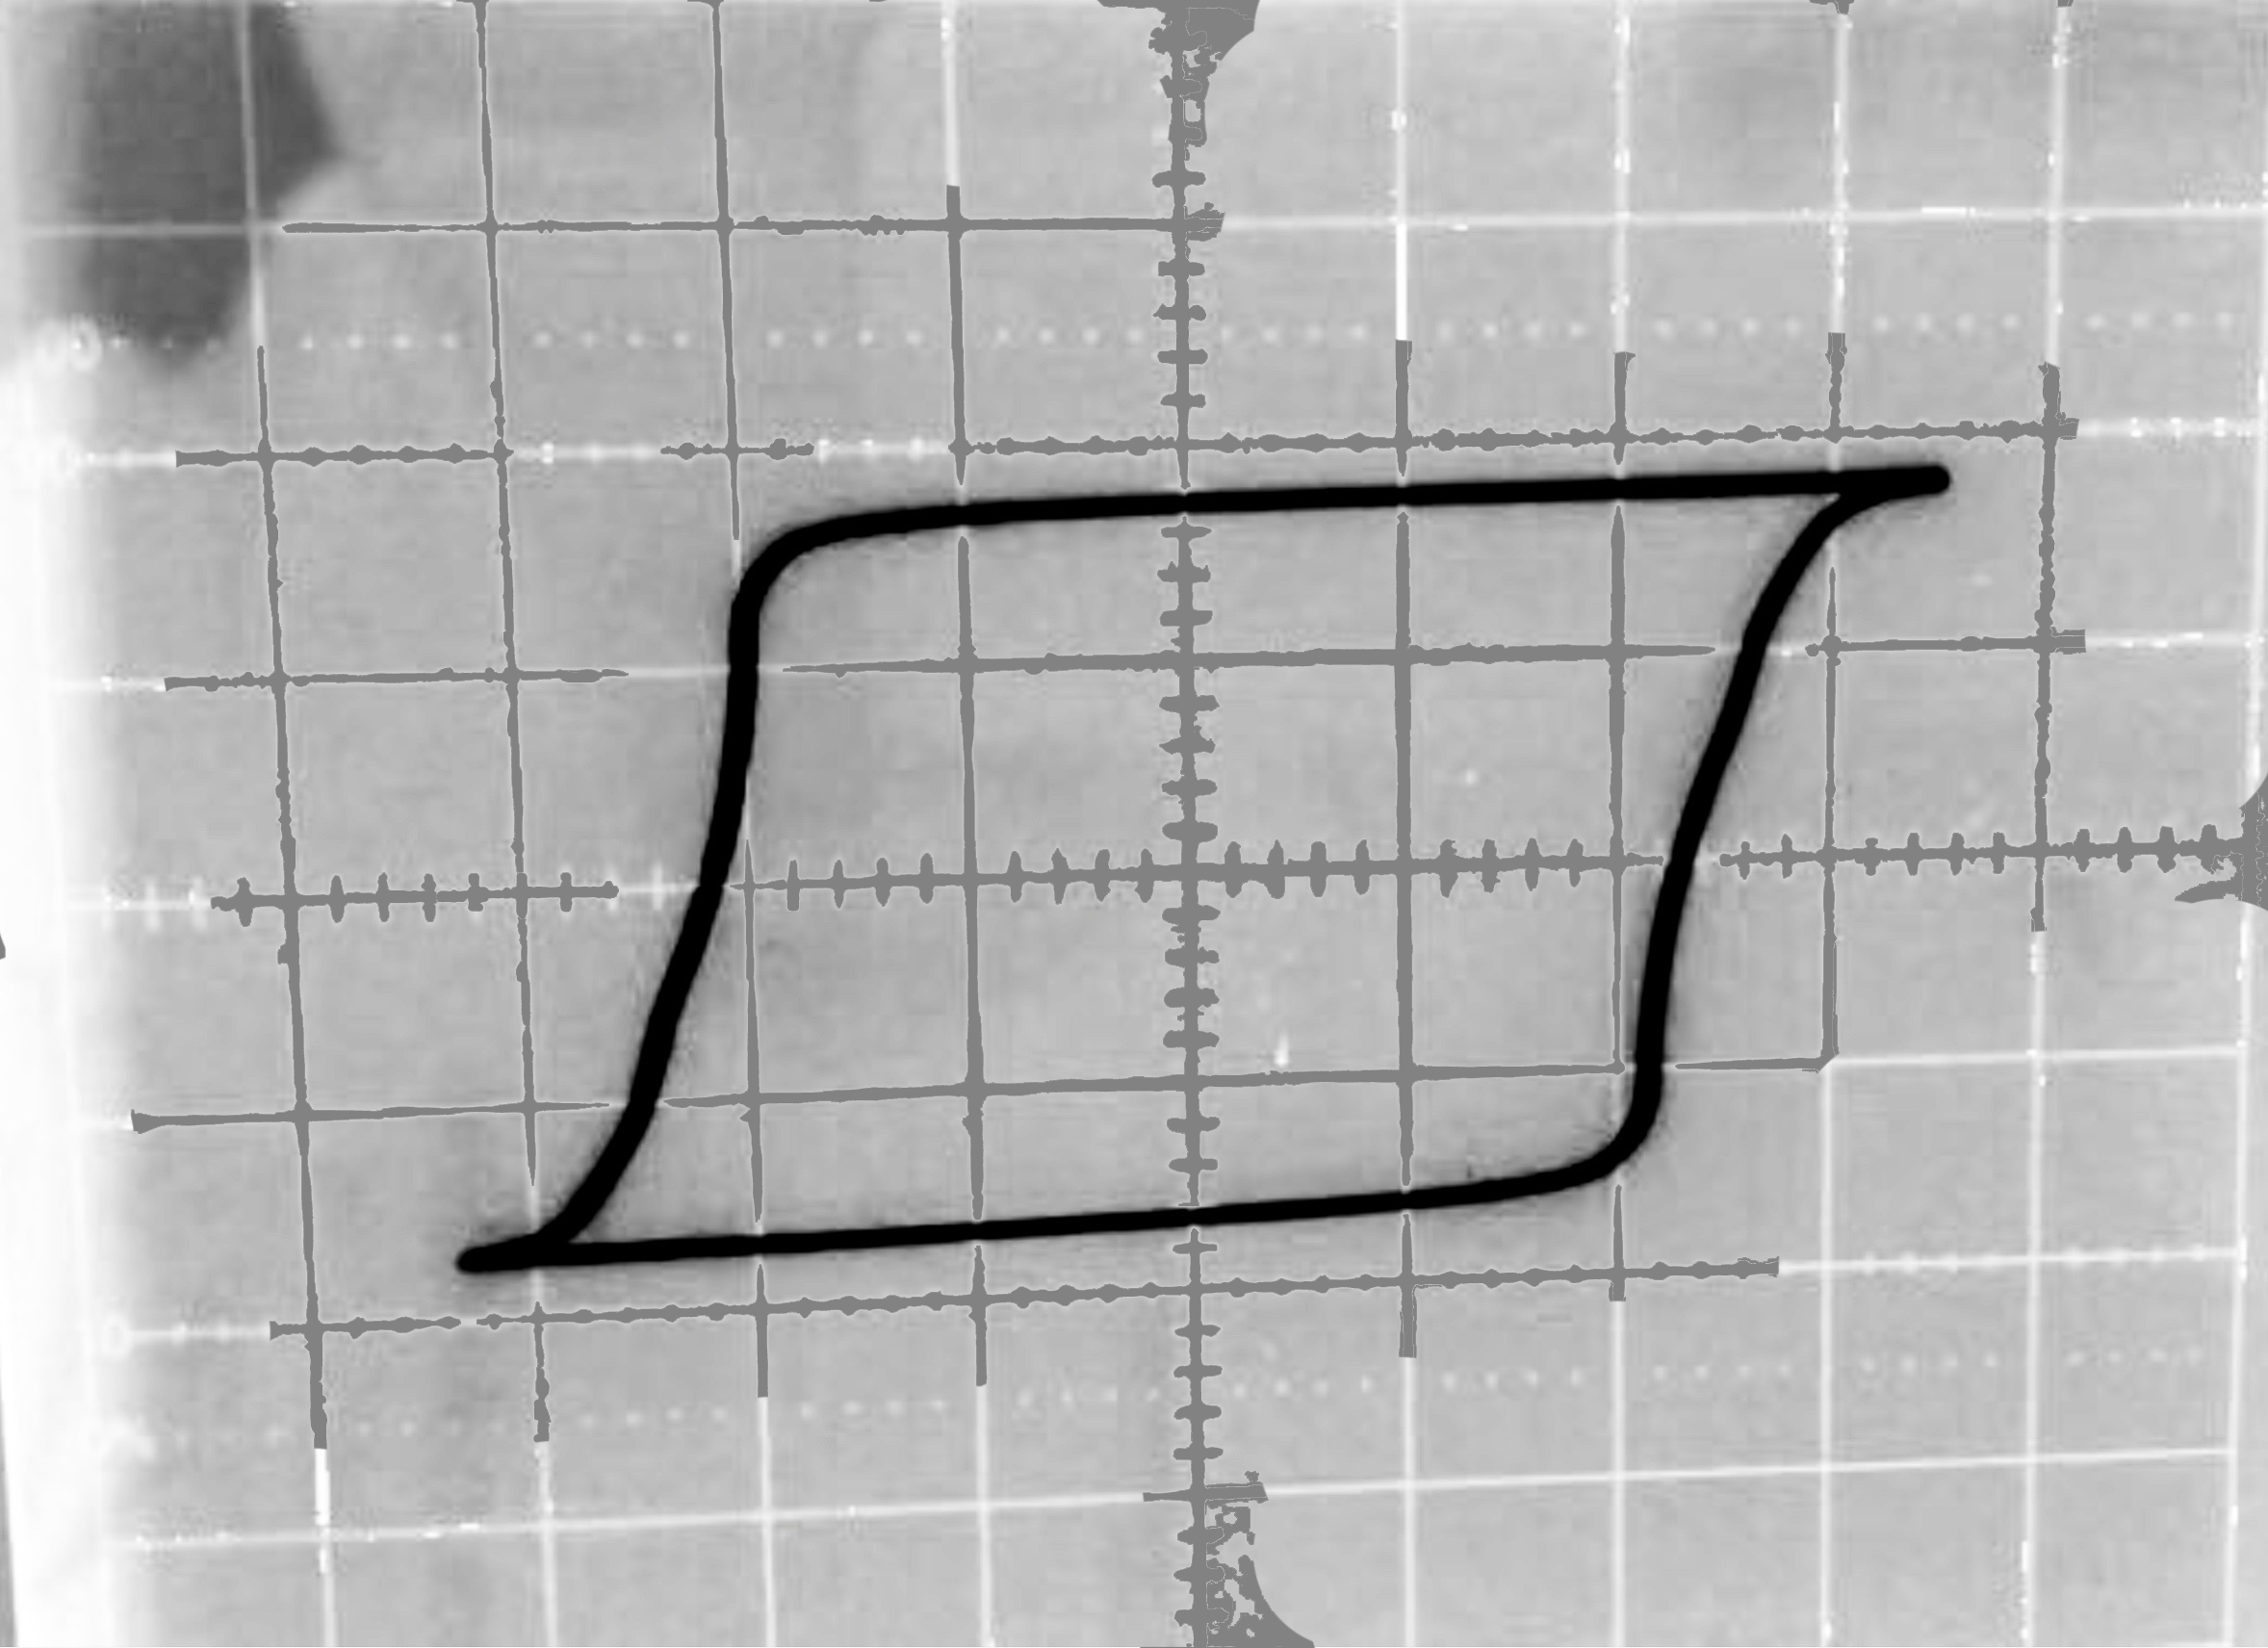
\includegraphics[scale=0.2]{2.png}
	\caption{Петля гистерезиса для пермаллоя}
\end{figure}

  		
  		\begin{table}[h!]
  		\caption{Начальная кривая намагничивания для феррита}
  		\begin{center}
  			\begin{tabular}{|c|c|c|c|c|c|c|c|c|c|c|c|c|c|} 
  				\hline 
  				№ &  1 &  2 & 3 & 4 & 5 &  6 &  7 & 8 & 9 & 10  &  11 &  12 &13   \\ 	\hline
  				
  			$ x $, дел &3.0 & 2.5 & 2.3 & 1.8 & 1.6 & 1.4 & 1.2 & 1.0 & 0.8 & 0.6 & 0.4 & 0.2 & 0.0 \\
  			 $ y $, дел & 3.6 & 3.4 & 3.3 & 3.1 & 3.0 & 2.7 & 2.4 & 2.2 & 2.0 & 1.2 & 0.5 & 0.2 & 0.0 \\
  				\hline
  				
  			\end{tabular}
  		\end{center}
  	\end{table}
  	
  	
  
  	\begin{figure}[h!]
  	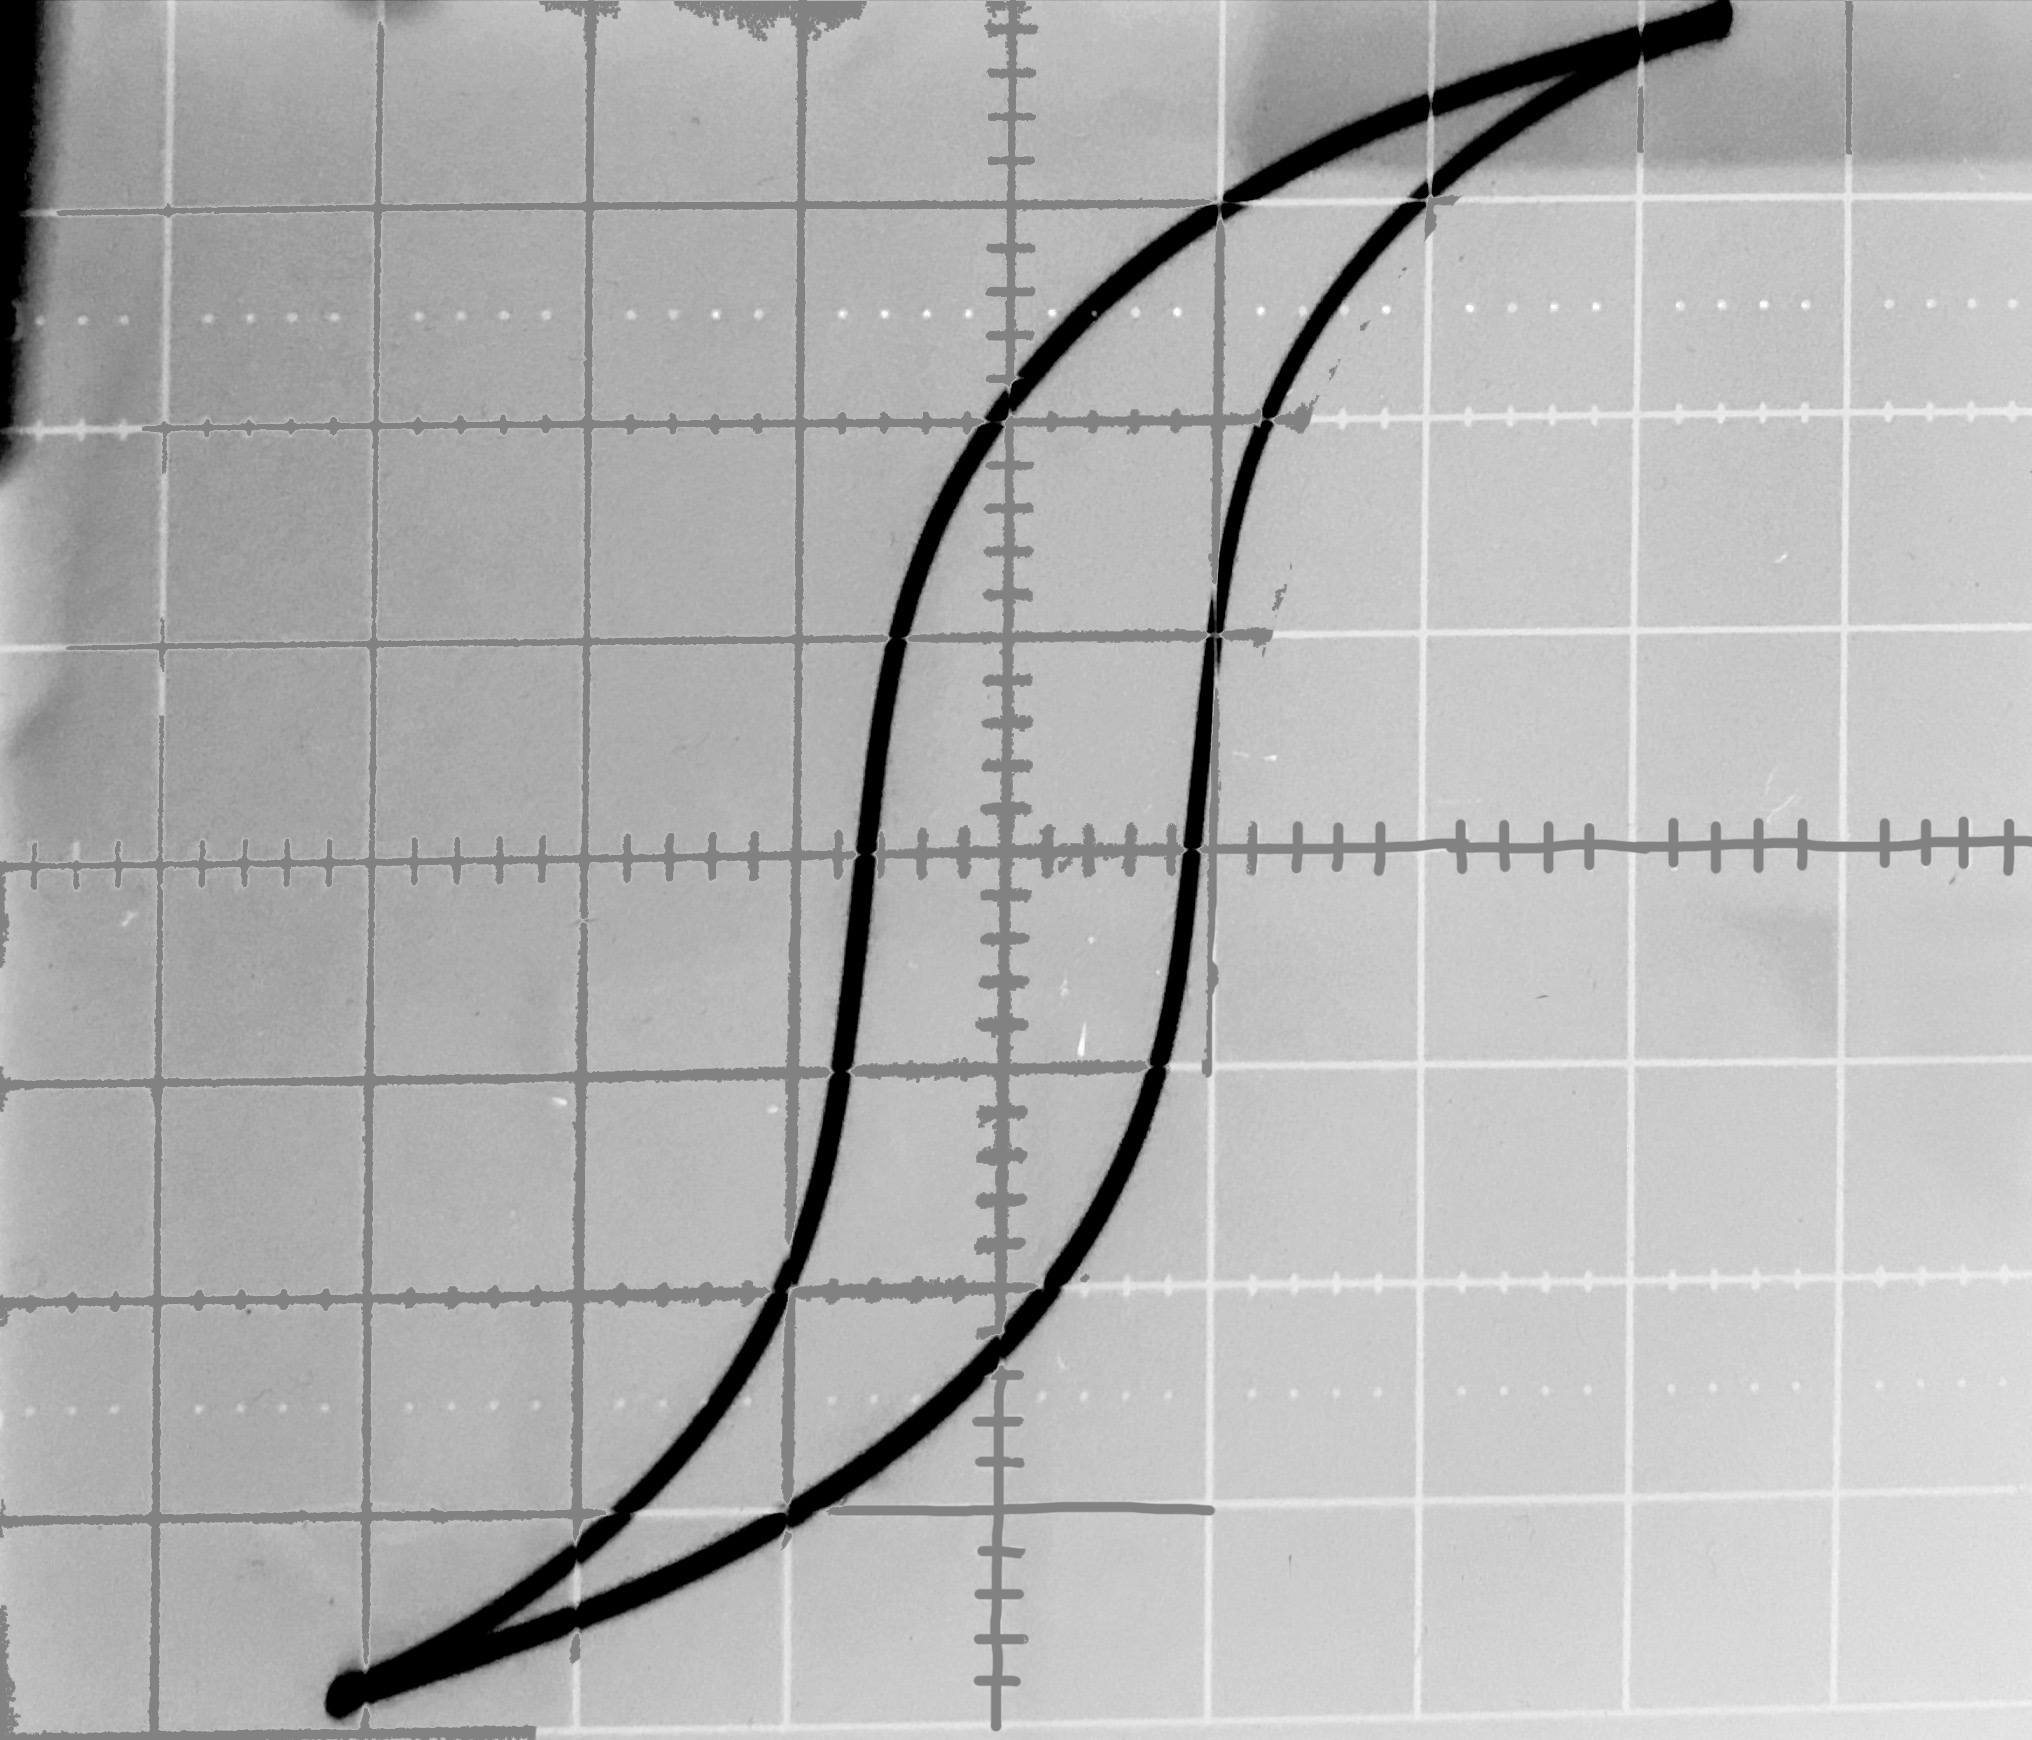
\includegraphics[scale=0.22]{3.png}
  	\caption{Петля гистерезиса для феррита}
  \end{figure}  			
  		

  	  
  	  	
  	  	
  	  	\item Восстановим предельные петли для образцов. Рассчитаем  цену деления ЭО для петли для оси Х (в $\dfrac{А}{м}$) по формуле
  	  	
  	  	$$H=\dfrac{IN_{0}}{2\pi R},$$
  	  	
  	  	где $I=\dfrac{K_{x}}{R_{0}}$, и в Теслах на деление для оси Y по формуле
  	  	
  	  	$$B=\dfrac{R_{и}С_{и}U_{вых}}{SN_{и}},$$
  	  	
  	  	где $U_{вых}=K_{y}.$
  	  	
  	  	
  		\begin{itemize}
  			\item \textbf{Кремниевое железо}:
  	  	
  	  	$H=90,9 \dfrac{А}{м}.$
  	  	$B=0,20 \dfrac{Т}{дел}.$
  	
  	\item	\textbf{Пермаллой}:
  	
  $H=10,6 \dfrac{А}{м}.$
  	$B=1,01 \dfrac{Т}{дел}.$
  	
  	\item	\textbf{Феррит}:
  		
  		$H=9,0 \dfrac{А}{м}.$
  		$B=3,33 \cdot 10^{-2} \dfrac{Т}{дел}.$
  	
  		\end{itemize}
 
  		
  		\item Соединим вход ячейки с обмоткой "<6,3 В"> трансформатора.
  		
  		 Определим входное напряжение на $ RC $-цепочке: $U_{вх}=2y\cdot K_{y} = 2 \x 7,2 = 14,4 $ В.
  		
  		Не меняя тока, переключим Y-вход ЭО к выходу ячейки и аналогичным образом определим $U_{вых} = 10 \x 10^{-3} \x 5,6 = 56 \x 10^{-3} $ В. 
  		
  		Определим $\tau = RC $ по формуле
  		
  		$$\tau = \dfrac{U_{вх}}{\Omega U_{вых}}=0,52 \pm 0,06 \; Ом\cdot Ф.$$
  		
  		Полученное значение $\tau \approx R_иC_и = 0,4 \ Ом\cdot Ф$.
  		
  		\item Рассчитаем коэрцитивную силу $H_{c}$ и индукцию насыщения $B_{s}$ для каждого образца.
  		
  	\begin{itemize}
  		\item 	\textbf{Кремниевое железо}:
  		
  		\fbox{$H_{c}=54,5 \pm 0,8 \dfrac{А}{м}$}
  		\fbox{$B_{s}=0,70 \pm 0,03 \ Тл$}
  		
  	\item	\textbf{Пермаллой}:
  		
  		\fbox{$H_{c}=24,4 \pm 0,5 \dfrac{А}{м}$}
  		\fbox{$B_{s}=1,82 \pm 0,06 \ Тл$}
  		
  	\item	\textbf{Феррит}:
  		
  		\fbox{$H_{c}=8,1 \pm 0,2 \dfrac{А}{м}$}
  		\fbox{$B_{s}=(12,9\pm 0,02) \cdot 10^{-2} Тл$}
 
 	\end{itemize}
  		
  		\newpage
  		
  		\item Из графиков (4-6) оценим максимальные значения дифференциальной магнитной проницаемости.
  		
  	\begin{itemize}
  		\item 	\textbf{Кремнистое железо}:
  		
  		\fbox{$\mu_{max} \simeq (30,6 \pm 2,9 ) \x 10^3 $}
  		
  	\item	\textbf{Пермаллой}:
  	
  		\fbox{$\mu_{max} \simeq (89,7 \pm 7,6) \x 10^3 $}
  		
  		\textbf{Феррит}:
  		
  	\item	\fbox{$\mu_{max} \simeq (7,6 \pm 0,6) \x 10^3$}
  		
  	\end{itemize}
  		
  	\end{enumerate}
\end{document}